\documentclass[border=10pt]{standalone}
\usepackage{tikz}
\usetikzlibrary{3d, calc, arrows.meta}

\begin{document}
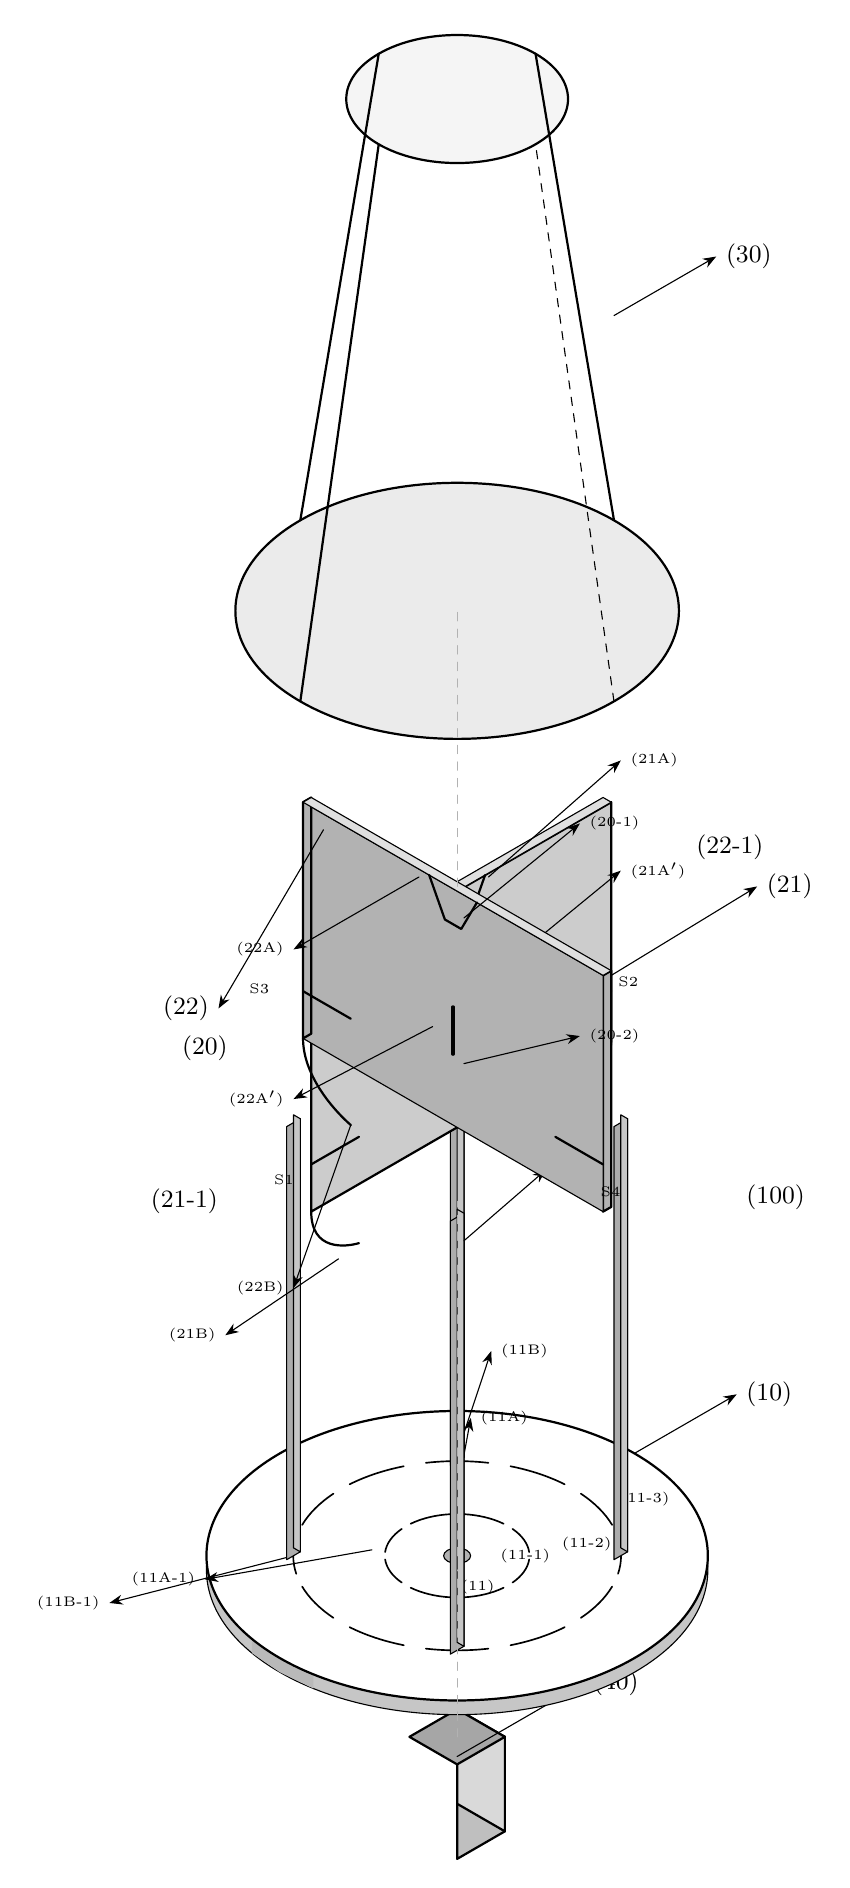
\begin{tikzpicture}[
  x={(0.866cm, 0.5cm)},
  y={(0cm, 1cm)},
  z={(-0.866cm, 0.5cm)},
  line join=round, line cap=round
]

% ── 분리 사시도 Y축 높이 설정 ──────────────────────────────
\def\yFeed{0}    % (40) 급전 커넥터
\def\yPlate{3.5} % (10) 접지 플레이트  ← 간격 확대
\def\yRad{9.0}   % (20) 방사 소자     ← 간격 확대
\def\yCover{15.5}% (30) 보호 커버     ← 간격 확대

% ══════════════════════════════════════════════════════════
% (40) 급전 커넥터 — 플레이트 하단에 결합되는 동축 커넥터
% ══════════════════════════════════════════════════════════
\def\FC{0.35}
\fill[gray!50, draw=black, thick]
  (-\FC,\yFeed,-\FC) -- (\FC,\yFeed,-\FC) -- (\FC,\yFeed+1.2,-\FC) -- (-\FC,\yFeed+1.2,-\FC) -- cycle;
\fill[gray!30, draw=black, thick]
  (\FC,\yFeed,-\FC) -- (\FC,\yFeed,\FC) -- (\FC,\yFeed+1.2,\FC) -- (\FC,\yFeed+1.2,-\FC) -- cycle;
\fill[gray!70, draw=black, thick]
  (-\FC,\yFeed+1.2,-\FC) -- (\FC,\yFeed+1.2,-\FC) -- (\FC,\yFeed+1.2,\FC) -- (-\FC,\yFeed+1.2,\FC) -- cycle;
\draw[->, >=Stealth, thin]
  (\FC,\yFeed+0.6,\FC) -- (2.2,\yFeed+0.6,\FC) node[right, font=\small] {(40)};

% ══════════════════════════════════════════════════════════
% (10) 접지 플레이트 — 슬롯(11A, 11B) 포함 사각 플레이트
% ══════════════════════════════════════════════════════════
\def\PR{2.6}   % 플레이트 반지름 (원형)
\def\PT{0.18}  % 두께
\def\rA{0.75}  % 내측 슬롯부(11A) 반경
\def\rB{1.7}   % 외측 슬롯부(11B) 반경

% 하면 (두께 표현용)
\begin{scope}[canvas is xz plane at y=\yPlate-\PT]
  \fill[gray!45, draw=black] (0,0) circle (\PR);
\end{scope}
% 외주 측면 (앞쪽 반원 가장자리)
\foreach \ang in {180,170,...,360} {
  \pgfmathsetmacro{\px}{\PR*cos(\ang)}
  \pgfmathsetmacro{\pz}{\PR*sin(\ang)}
  \pgfmathsetmacro{\qx}{\PR*cos(\ang+10)}
  \pgfmathsetmacro{\qz}{\PR*sin(\ang+10)}
  \fill[gray!55, draw=none]
    (\px,\yPlate-\PT,\pz) -- (\qx,\yPlate-\PT,\qz)
    -- (\qx,\yPlate,\qz) -- (\px,\yPlate,\pz) -- cycle;
}
% 상면
\begin{scope}[canvas is xz plane at y=\yPlate]
  \fill[white, draw=black, thick] (0,0) circle (\PR);
\end{scope}

% 슬롯
\begin{scope}[canvas is xz plane at y=\yPlate]
  % 내측 슬롯부 (11A): 원호상 구멍 8개
  \foreach \k in {0,...,7} {
    \pgfmathsetmacro{\s}{\k*45+5}
    \draw[semithick] (\s:\rA) arc (\s:\s+35:\rA);
  }
  % 외측 슬롯부 (11B): 원호상 구멍 12개
  \foreach \k in {0,...,11} {
    \pgfmathsetmacro{\s}{\k*30+4}
    \draw[semithick] (\s:\rB) arc (\s:\s+22:\rB);
  }
  % 중앙 구멍
  \fill[gray!60, draw=black] (0,0) circle (0.14);
\end{scope}

% 슬롯 레이블 — 플레이트 표면 위에서 깔끔하게 인출
% (11A): 내측 슬롯 → 우전방
\draw[->, >=Stealth, thin]
  (0.55,\yPlate,0.6) -- (1.8,\yPlate+0.05,1.6) node[right, font=\tiny] {(11A)};
% (11B): 외측 슬롯 → 우전방 더 멀리
\draw[->, >=Stealth, thin]
  (1.3,\yPlate,1.3) -- (2.8,\yPlate+0.05,2.3) node[right, font=\tiny] {(11B)};
% (11A-1)(11B-1): 개별 구멍 → 좌후방
\draw[->, >=Stealth, thin]
  (-0.55,\yPlate,0.7) -- (-2.2,\yPlate+0.05,1.5) node[left, font=\tiny] {(11A-1)};
\draw[->, >=Stealth, thin]
  (-1.2,\yPlate,1.2) -- (-3.2,\yPlate+0.05,1.9) node[left, font=\tiny] {(11B-1)};
% 중앙 / 반경방향 구역 레이블 — 우후방 (비어있는 공간)
\node[font=\tiny] at (-0.25,\yPlate,-0.55) {(11)};
\node[font=\tiny] at (0.5,\yPlate,-0.5)  {(11-1)};
\node[font=\tiny] at (1.1,\yPlate,-0.8)  {(11-2)};
\node[font=\tiny] at (2.1,\yPlate,-0.65) {(11-3)};

% 플레이트 인출선
\draw[->, >=Stealth, thin]
  (\PR,\yPlate,0) -- (\PR+1.5,\yPlate,0) node[right, font=\small] {(10)};

% ══════════════════════════════════════════════════════════
% (50~53) 절연 지지대 — 4개 기둥
% ══════════════════════════════════════════════════════════
\def\SH{0.1}
\foreach \sx/\sz in {1.2/1.2, -1.2/1.2, 1.2/-1.2, -1.2/-1.2} {
  \fill[gray!65, draw=black]
    (\sx-\SH,\yPlate,\sz) -- (\sx+\SH,\yPlate,\sz) --
    (\sx+\SH,\yRad,\sz) -- (\sx-\SH,\yRad,\sz) -- cycle;
  \fill[gray!45, draw=black]
    (\sx+\SH,\yPlate,\sz) -- (\sx+\SH,\yPlate,\sz+\SH) --
    (\sx+\SH,\yRad,\sz+\SH) -- (\sx+\SH,\yRad,\sz) -- cycle;
}
\pgfmathsetmacro{\ySupMid}{(\yPlate+\yRad)/2}
% 지지대 레이블 — 오른쪽 기둥에서 인출
\draw[->, >=Stealth, thin]
  (1.3,\ySupMid,1.2) -- (2.8,\ySupMid,1.5) node[right, font=\tiny] {(50)};

% ══════════════════════════════════════════════════════════
% (20) 방사 소자 — 십자형 동박판
% ══════════════════════════════════════════════════════════
\def\RW{2.2}   % 방사 소자 반폭
\def\RH{3.0}   % 방사 소자 높이
\def\RT{0.06}  % 박판 반두께

% ── 가로 방사 소자 (21): X 방향 ──
\fill[white!80!black, draw=black, thick]
  (-\RW,\yRad,-\RT) -- (\RW,\yRad,-\RT) -- (\RW,\yRad+\RH,-\RT) -- (-\RW,\yRad+\RH,-\RT) -- cycle;
\fill[gray!25, draw=black]
  (-\RW,\yRad+\RH,-\RT) -- (\RW,\yRad+\RH,-\RT) -- (\RW,\yRad+\RH,\RT) -- (-\RW,\yRad+\RH,\RT) -- cycle;
% 하방 만곡부
\draw[thick]
  (-\RW,\yRad,-\RT) .. controls (-\RW,\yRad-0.5,-\RT) and (-\RW+0.5,\yRad-0.7,-\RT)
  .. (-\RW+0.7,\yRad-0.75,-\RT);
\draw[thick]
  (\RW,\yRad,-\RT) .. controls (\RW,\yRad-0.5,-\RT) and (\RW-0.5,\yRad-0.7,-\RT)
  .. (\RW-0.7,\yRad-0.75,-\RT);
% 슬릿 (S1, S2)
\draw[thick] (-\RW,\yRad+0.6,-\RT) -- (-\RW+0.7,\yRad+0.6,-\RT);
\draw[thick] (\RW-0.7,\yRad+0.6,-\RT) -- (\RW,\yRad+0.6,-\RT);
\node[font=\tiny] at (-\RW-0.4,\yRad+0.6,-\RT) {S1};
\node[font=\tiny] at (\RW+0.25,\yRad+0.6,-\RT) {S2};

% 중앙 요입부(21A)
\draw[thick] (-0.35,\yRad+\RH,-\RT) -- (-0.12,\yRad+\RH-0.45,-\RT)
  -- (0.12,\yRad+\RH-0.45,-\RT) -- (0.35,\yRad+\RH,-\RT);
% 끼움 절결부(21A')
\draw[very thick] (0,\yRad+\RH-0.45,-\RT) -- (0,\yRad+\RH/2,-\RT);

% 가로 소자 레이블 — (21A): 상단 우측 인출, (21A'): 중단 우측 인출
\draw[->, >=Stealth, thin]
  (0.4,\yRad+\RH-0.05,-\RT) -- (2.4,\yRad+\RH+0.4,0) node[right, font=\tiny] {(21A)};
\draw[->, >=Stealth, thin]
  (0.15,\yRad+\RH/2+0.1,-\RT) -- (2.4,\yRad+\RH/2+0.5,0) node[right, font=\tiny] {(21A$'$)};
% 하방 만곡부·본체 레이블 — 왼쪽 공간
\draw[->, >=Stealth, thin]
  (-\RW+0.4,\yRad-0.8,-\RT) -- (-\RW-1.2,\yRad-1.0,0) node[left, font=\tiny] {(21B)};
\node[font=\small] at (-\RW-1.8,\yRad+\RH/2-0.5,0) {(21-1)};

% ── 세로 방사 소자 (22): Z 방향 ──
\fill[white!70!black, draw=black, thick]
  (-\RT,\yRad,-\RW) -- (\RT,\yRad,-\RW) -- (\RT,\yRad+\RH,-\RW) -- (-\RT,\yRad+\RH,-\RW) -- cycle;
\fill[white!70!black, draw=black]
  (-\RT,\yRad,-\RW) -- (-\RT,\yRad,\RW) -- (-\RT,\yRad+\RH,\RW) -- (-\RT,\yRad+\RH,-\RW) -- cycle;
\fill[white!70!black, draw=black, thick]
  (-\RT,\yRad,\RW) -- (\RT,\yRad,\RW) -- (\RT,\yRad+\RH,\RW) -- (-\RT,\yRad+\RH,\RW) -- cycle;
\fill[gray!25, draw=black]
  (-\RT,\yRad+\RH,-\RW) -- (-\RT,\yRad+\RH,\RW) -- (\RT,\yRad+\RH,\RW) -- (\RT,\yRad+\RH,-\RW) -- cycle;
% 하방 만곡부
\draw[thick]
  (-\RT,\yRad,\RW) .. controls (-\RT,\yRad-0.5,\RW) and (-\RT,\yRad-0.7,\RW-0.5)
  .. (-\RT,\yRad-0.75,\RW-0.7);
% 슬릿 (S3, S4)
\draw[thick] (-\RT,\yRad+0.6,-\RW) -- (-\RT,\yRad+0.6,-\RW+0.7);
\draw[thick] (-\RT,\yRad+0.6,\RW-0.7) -- (-\RT,\yRad+0.6,\RW);
\node[font=\tiny] at (-0.35,\yRad+0.6,\RW+0.35) {S3};
\node[font=\tiny] at (-0.35,\yRad+0.6,-\RW-0.4) {S4};

% 중앙 요입부(22A)
\draw[thick] (-\RT,\yRad+\RH,-0.35) -- (-\RT,\yRad+\RH-0.45,-0.12)
  -- (-\RT,\yRad+\RH-0.45,0.12) -- (-\RT,\yRad+\RH,0.35);
% 끼움 절결부(22A')
\draw[very thick] (-\RT,\yRad+0.9,0) -- (-\RT,\yRad+\RH/2,0);

% 세로 소자 레이블 — Z+ 면 앞쪽에서 좌측으로 인출
\draw[->, >=Stealth, thin]
  (-\RT,\yRad+\RH-0.1,0.5) -- (-2.4,\yRad+\RH+0.4,0) node[left, font=\tiny] {(22A)};
\draw[->, >=Stealth, thin]
  (-\RT,\yRad+1.1,0.3) -- (-2.4,\yRad+1.5,0) node[left, font=\tiny] {(22A$'$)};
\draw[->, >=Stealth, thin]
  (-\RT,\yRad-0.75,\RW-0.7) -- (-2.4,\yRad-0.9,0) node[left, font=\tiny] {(22B)};
% (22-1) — 오른쪽 (21) 바로 위
\node[font=\small] at (\RW+1.8,\yRad+\RH/2,0) {(22-1)};

% ── 방사 소자 주요 인출선 ──
% (21) — 오른쪽 중단 (가장 외곽, 22-1보다 아래)
\draw[->, >=Stealth, thin]
  (\RW,\yRad+0.8,-\RT) -- (\RW+2.2,\yRad+0.8,0) node[right, font=\small] {(21)};
% (22) — Z+ 면 상단 모서리에서 좌측 인출
\draw[->, >=Stealth, thin]
  (-\RT,\yRad+2.8,\RW-0.3) -- (-3.5,\yRad+3.2,0) node[left, font=\small] {(22)};
% (20) — 왼쪽 중단 (21-1보다 위)
\node[font=\small] at (-\RW-1.5,\yRad+\RH-0.2,0) {(20)};

% 연결 부재 (20-1 상부, 20-2 하부) — 높이 차이를 두어 구분
\draw[->, >=Stealth, thin]
  (0.2,\yRad+\RH-0.55,0.1) -- (1.8,\yRad+\RH-0.1,0) node[right, font=\tiny] {(20-1)};
\draw[->, >=Stealth, thin]
  (0.2,\yRad+0.60,0.1) -- (1.8,\yRad+0.20,0) node[right, font=\tiny] {(20-2)};

% ══════════════════════════════════════════════════════════
% (30) 보호 커버 — 원통형
% ══════════════════════════════════════════════════════════
\def\CR{2.3}   % 커버 반지름
\def\CL{6.5}   % 커버 높이

\begin{scope}[canvas is xz plane at y=\yCover]
  \fill[white!92!black, draw=black, thick] (0,0) circle (\CR);
\end{scope}
\begin{scope}[canvas is xz plane at y=\yCover+\CL]
  \fill[white!96!black, draw=black, thick] (0,0) circle (\CR*0.5);
\end{scope}
% 측면 수직선
\draw[thick] ( \CR,\yCover,0) -- ( \CR*0.5,\yCover+\CL,0);
\draw[thick] (-\CR,\yCover,0) -- (-\CR*0.5,\yCover+\CL,0);
\draw[thick] (0,\yCover, \CR) -- (0,\yCover+\CL, \CR*0.5);
\draw[dashed](0,\yCover,-\CR) -- (0,\yCover+\CL,-\CR*0.5);

\draw[->, >=Stealth, thin]
  (\CR,\yCover+\CL*0.4,0) -- (\CR+1.5,\yCover+\CL*0.4,0) node[right, font=\small] {(30)};

% ══════════════════════════════════════════════════════════
% 분리 가이드선 (폭발도 중심축)
% ══════════════════════════════════════════════════════════
\draw[dashed, gray!60, thin] (0,\yFeed+1.2,0) -- (0,\yPlate-\PT,0);
\draw[dashed, gray!60, thin] (0,\yPlate,0)    -- (0,\yRad-1.0,0);
\draw[dashed, gray!60, thin] (0,\yRad+\RH,0)  -- (0,\yCover,0);

% ══════════════════════════════════════════════════════════
% 전체 안테나 참조번호 (100)
% ══════════════════════════════════════════════════════════
\node[font=\small, anchor=west] at (\PR+1.5,\yPlate+2.5,0) {(100)};

\end{tikzpicture}
\end{document}
